\chapter{Uniprocessor Scheduling}
\section{4 Scheduling Methods}
Målet med scheduling er å tilegne prosesser rett til "execution" slik at vi imøtekommer kravet om responstid, "througput", og prosessor effektivitet. 
Four types of scheduling er nevnt i dette kap. 
\begin{itemize}
\item 
\emph{Long term scheduling} - der vi har en gatekeeper som avgjør om nye oppgaver skal legges til i minne. Den begrenser multitasking til fordel for raskere kjøring.
\item 
\emph{Medium term scheduling} - her velger vi om en oppgave skal kjøres eller settes i vent. Når pcen er mindre busy så kan de ventende oppgavene kjøre.
\item 
\emph{Short term scheduling }- tar en jobb fra "ready" og gir den grønt lys til å kjøre. Den avgjør hvor lenge hver tråd kan oppta en ressurs. 
\item 
\emph{I/O scheduling }- En sentral faktor i alle operativsystemers design omfatter håndtering av prosesser og tråder: 
\end{itemize}

Det finnes not å utdype seg i når det gjelder disse fire scheduling metodene. Et kriteria variere mello ulike systemer, se listen \ref{fig:critera_sc} nedenfor for å se variasjonene. 

\begin{figure}
\centering
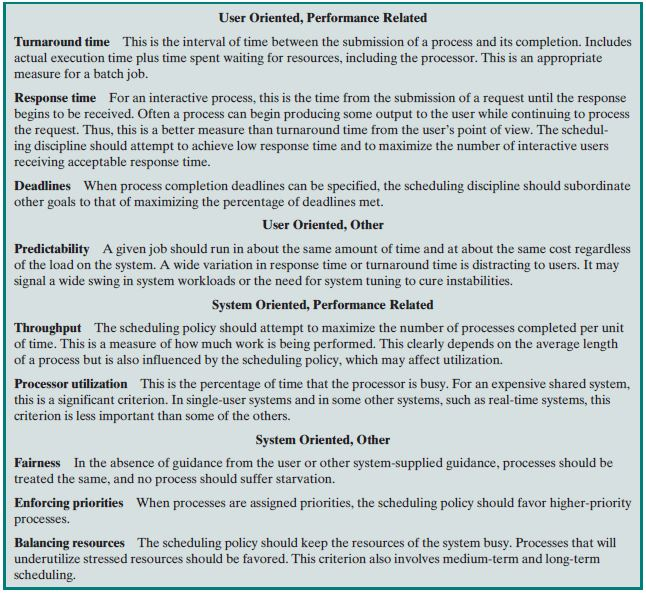
\includegraphics{img/scheduling.JPG}
\caption{Scheduling Criteria}
\label{fig:critera_sc}
\end{figure}

\newpage
\section{Priorities}
I mange systemer har hver prosess fått signert en prioritet, høyere prioritet velges alltid over lavere prioritet. Her kan man for enkelthetskyld tenke seg flere paralelle køer (queues). Som samtidig blir sortert etter prioritet.
Tabell \ref{fig:schedule_po} presenterer en oppsumering av de forskjellig schedulingmetodene som vi skal gå gjennom nå. 
\subsubsection{}
w = time spent in system so far, waiting\newline
e = time spent in extution so far\newline
s = total service time required by the process, including e; generally, this quantity must be estimated or supplied by the user.\newline\newline

\begin{figure}
\centering
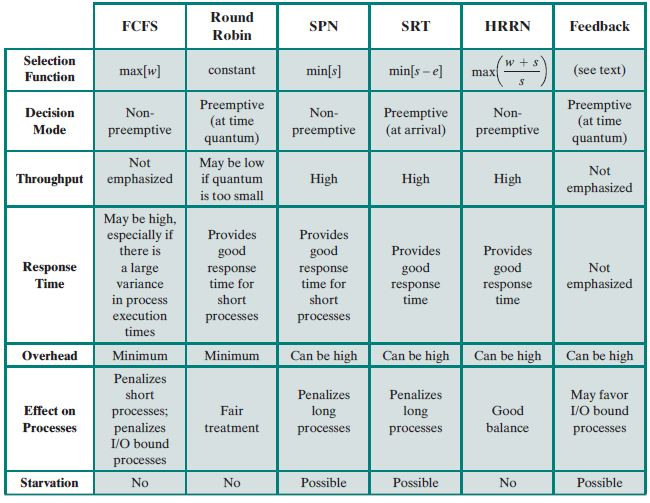
\includegraphics{img/scheduling_policy.JPG}
\caption{Scheduling Policies}
\label{fig:schedule_po}
\end{figure}

Anta at vi har prosessene i figur \ref{fig:schedule_ex}. Disse skal gå gjennom forskellige sceduling metoder som i figur \ref{fig:schedule_alg}. Stikk en side ned og finn figuren, så kan du begynne på Scheduling Algoriths.

\begin{figure}[h!]
\centering
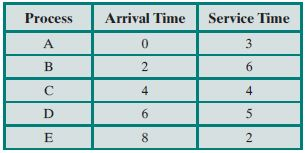
\includegraphics{img/schedule_ex.JPG}
\caption{sceduling example}
\label{fig:schedule_ex}
\end{figure}

\begin{figure}[h!]
\centering
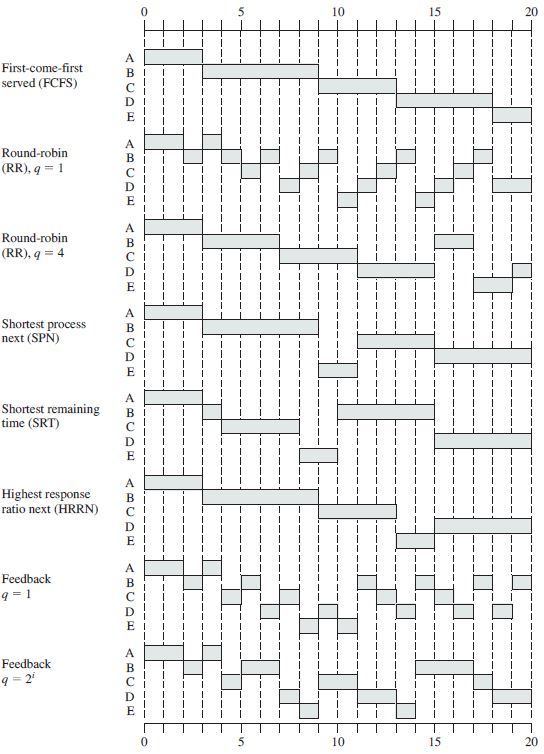
\includegraphics{img/schedule_alg.JPG}
\caption{Scheduling Algorithms}
\label{fig:schedule_alg}
\end{figure}

\FloatBarrier
\section{Scheduling Algorithms}
\subsubsection{FIRST COME FIRST SERVE aka (FIFO)}
Det kan være en god ide å teste seg litt på eksemplene i figur \ref{fig:schedule_alg}. De enklese å forstå er naturligvis FCFS og Round-robin. Når det gjelder ulemper med FCFS/FIFO så har den en tendens til å favorisere prosessor bundet prosesser. Se for deg en haug med prosesser, en av dem er prosessor bundet, de andre er I/O bundet. Alle I/O prosessene er i wait, noen av dem er kanskje "blocket" fordi de venter på I/O, men noen kan plutselig få klarsignal. Selv om det er potensilt arbeid for dem å gjøre (DMA, lese, skrive, osv), så blir de ikke satt igang. FIFO er ikke populert på "uniprosessor" systemer. Men kan bli bedre med prioritetskø. 
\subsubsection{ROUND ROBIN}
En enklere måte å komme gjennom penalty slik som FIFO er å bruke preemption basert på systemklokke. Den enkleste heter round robin. Et klokke interrupt genereres periodisk. Denne teknikken kalles også \emph{"Time Slicing"}. En ulempe med dette systemet er overhead ved interrupt. Et annet problem er at prosessor bundet prosesser har en tendens til å få ufordelaktige porsjoner av prosessortiden. 
Det ble foreslått en endring til round robin, når en I/O prosess blokkeres så legges den i en I/O kø. Slik som vanlig round robin, men etter det blir den lagt inn i en auxiliary kø, her får den prioritet over hovedkøen. Herfra kjøres den på prosessoren i en basistid minus den totale tiden den brukte på å kjøre siden sist den ble selektert i hovedkøen. Siste bit er kanskje litt komplisert, men se om det sitter igjen til eksamen. Det viser seg at performance messig så er den nye løsningen fordelaktig til vanlig round robin.  
\subsubsection{Shortest Process Next}
Dette er en nonpreemtive "policy", der prosessen med kortest kjøretid blir fordelt prosessortid. Den totale kjøretiden med hensyn på responstid blir "significantly" bedre. Men variasjonen på responstid blir større. Et problem er at du trenger å vite kjøretiden (Evt estimere). For batchjobber må programmereren selv putte inn kjøretiden. I produksjonmiljøer så kommer jobber gjentatte ganger, slik er kalkulasjonen: Nå kommer det noen mattestykker, disse burde bli gitt på eksamen om du får en slik oppgave, men kan være greit å ha sett dem i sammenheng først, se derfor figur \ref{fig:spn}.

\begin{figure}[h!]
\centering
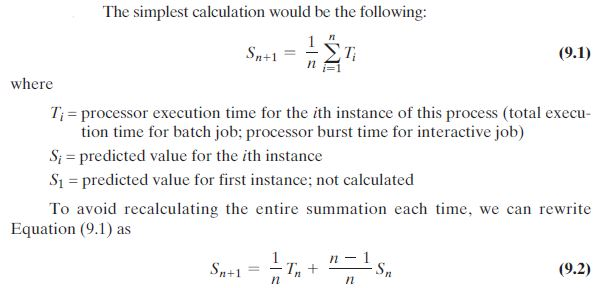
\includegraphics{img/SPN.JPG}
\caption{Shortest Process calculations from the book}
\label{fig:spn}
\end{figure}


For at et operativsysteme skal ha sjanse til å oppnå "concurrency" så må den som minstekrav støtte "mutual exclusion".